\documentclass[tikz]{standalone}

\usetikzlibrary{shapes.geometric, arrows}
\tikzstyle{startstop} = [rectangle, rounded corners, minimum width=3cm, minimum height=1cm,text centered, draw=black] % fill=red!30
\tikzstyle{io} = [trapezium, trapezium left angle=70, trapezium right angle=110, minimum width=3cm, minimum height=1cm, text centered, draw=black] % fill=blue!30
\tikzstyle{process} = [rectangle, minimum width=3cm, minimum height=1cm, text centered, text width=4cm, draw=black] % fill=orange!30
\tikzstyle{decision} = [diamond, minimum width=3cm, minimum height=1cm, text centered, draw=black] % fill=green!30
\tikzstyle{arrow} = [thick,->,>=stealth]

\begin{document}
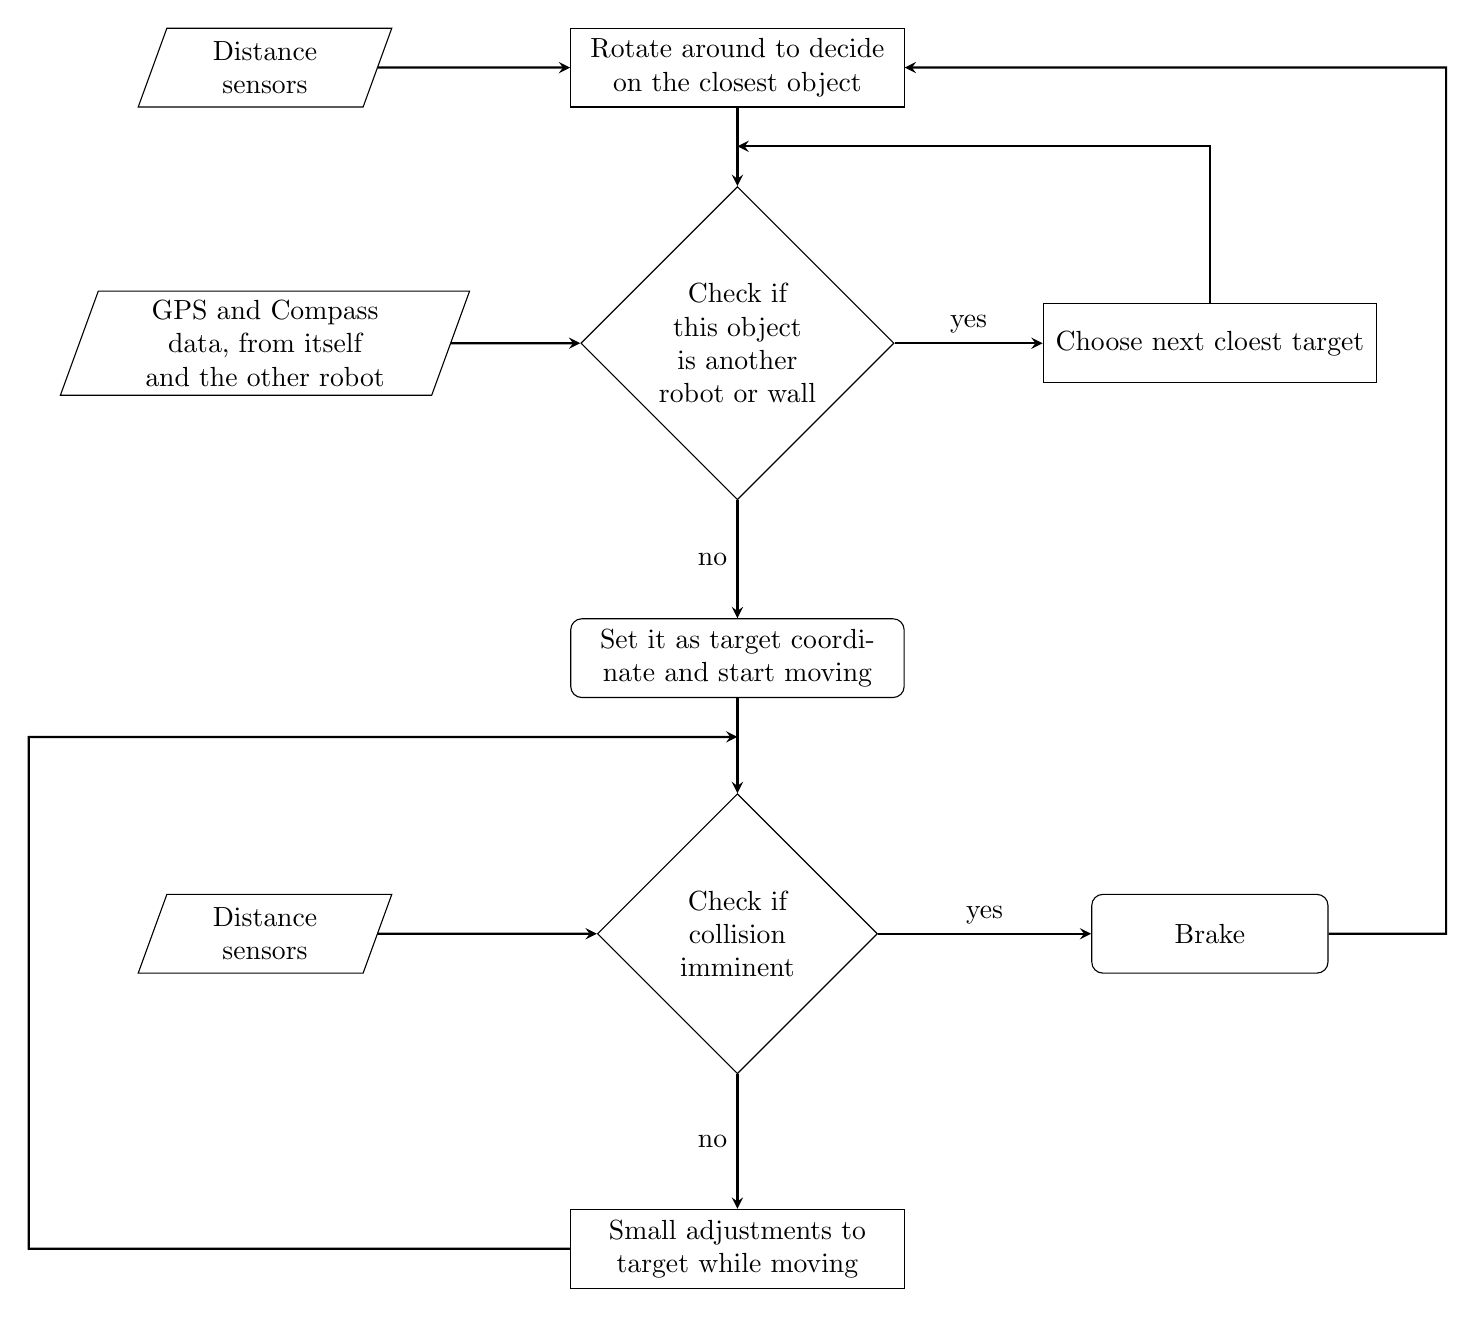
\begin{tikzpicture}[node distance=2cm]
\node (start) [process] {Rotate around to decide on the closest object};
\node (info1) [io, left of=start, xshift=-4cm, text width=2cm] {Distance sensors};

\node (dec1) [decision, below of=start, yshift=-1.5cm, text width=2cm] {Check if this object is another robot or wall};
\node (info2) [io, left of=dec1, xshift=-4cm, text width=4cm] {GPS and Compass data, from itself and the other robot};
\node (no) [startstop, below of=dec1, yshift=-2cm, text width=4cm] {Set it as target coordinate and start moving};
\node (yes) [process, right of=dec1, xshift=4cm] {Choose next cloest target};

\node (dec2) [decision, below of=no, yshift=-1.5cm, text width=2cm] {Check if collision imminent};
\node (info3) [io, left of=dec2, xshift=-4cm, text width=2cm] {Distance sensors};
\node (no2) [process, below of=dec2, yshift=-2cm] {Small adjustments to target while moving};
\node (yes2) [startstop, right of=dec2, xshift=4cm] {Brake};


\draw [arrow] (start) -- (dec1);
\draw [arrow] (info1) -- (start);
\draw [arrow] (info2) -- (dec1);
\draw [arrow] (dec1) -- node[left] {no} (no);
\draw [arrow] (dec1) -- node[above] {yes} (yes);
\draw [arrow] (yes) |- (0, -1cm);
\draw [arrow] (no) -- (dec2);
\draw [arrow] (info3) -- (dec2);
\draw [arrow] (dec2) -- node[above] {yes} (yes2);
\draw [arrow] (dec2) -- node[left] {no} (no2);
\draw [arrow] (yes2) -- (9cm, -11cm) |- (start);
\draw [arrow] (no2) -- (-9cm, -15cm) -- (-9cm, -8.5cm) -- (0, -8.5cm);

\end{tikzpicture}
\end{document}
